\chapter{Środowisko testowe}
W celu uniknięcia konieczności zajmowania się niskopoziomowymi problemami, takimi jak:
\begin{itemize}
    \item zrównoleglanie obliczeń wektorowych,
    \item wykonywanie obliczeń na~karcie graficznej,
    \item liczenie gradientów operacji wykonywanych przez sieć neuronową (takich jak~sploty, normalizacje, aktywacje),
    \item wczytywanie danych.
\end{itemize}
postanowiono skorzystać z~jednej~z~dostępnych bibliotek, która zajmuje się~owymi zagadnieniami. Pozwala to~na~skupienie
się~na~architekturze sieci oraz na~odpowiednim doborze operacji mających na~celu zapewnienie jak~najlepszej
klasyfikacji.

\section{Przegląd dostępnych narzędzi}
\subsection{Caffee}
Jedną z~najbardziej popularnych bibliotek wykorzystywanych w~głębokim uczeniu jest \textbf{Caffee} stworzona
i~rozwijana przez Berkeley Vision and~Learning Center (BVLC). Szczególnie często używana jest ona do~badań i~tworzenia
prototypów mechanizmów sztucznej inteligencji, które później implementowane są przy~wykorzystaniu innych narzędzi.
Samo Caffee umożliwia definiowanie architektury sieci poprzez pliki \textit{*.prototxt}, gdzie dane zapisane są
w notacji przypominającej JSON (\textit{ang.~JavaScript Object Notation}).

Choć Caffee nie~jest biblioteką Pythona, to~dostarcza narzędzi umożliwiających używanie jej z~poziomu tego języka.
Typowo wykorzystywane jest to~do~uruchamiania nauczonej już~sieci w~środowisku produkcyjnym, a~czasami
do~przeprowadzenia procesu uczenia w~środowiskach takich jak~chmury obliczeniowe. Istnieją również narzędzia,
dzięki którym możliwe jest używanie Caffee z~poziomu innych języków programowania np.~z~Matlaba.

Jedną z~zalet omawianej biblioteki jest również jej~szybkość. To~co~jednak zniechęca do~jej~zastosowania, to~ograniczone
możliwości stosowania niestandardowych zmian w~architekturze.

\subsection{Theano}
\textbf{Theano} to~jedna ze~starszych bibliotek wykorzystywanych do~konstrukcji mechanizmów głębokiego uczenia.
Jest to~biblioteka stworzona dla~języka Python, której głównymi celami są: definiowanie, optymalizacja i~obliczanie
wyrażeń matematycznych wykorzystujących tablice wielowymiarowe. Narzędzie do~osiągnięcia wymienionych zadań wykorzystuje
operacje przeprowadzane na~karcie graficznej, co~znacząco zwiększa wydajność obliczeń.

Wadą omawianej biblioteki jest to,~że~nie~definiuje ona złożonych operacji typowo wykorzystywanych w~sieciach
neuronowych, stąd~jest dość mało rozbudowana. Należy jednak wspomnieć, że~wiele narzędzi korzysta z~wzorców
wypracowanych podczas tworzenia Theano (np.~przenoszenie obliczeń na~kartę graficzną, definiowanie operacji na~zmiennych
symbolicznych itp.).

\subsection{Tensorflow}
TODO krótki opis Tensorflow
krótkie porównanie Caffe vs. Tensorflow (może tabelka??)

Do~realizacji badań wykonywanych w~ramach niniejszej pracy magisterskiej wykorzystano bibliotekę
\textbf{Tensorflow}.

W~kolejnym podrozdziale opisano podstawowe zagadnienia dotyczące wybranego narzędzia. Wiedza ta~pozwoli na~zrozumienie
informacji o~architekturze sieci przedstawianych w~dalszych częściach pracy.

\section{Graf operacji}
Tworzenie sztucznej sieci neuronowowej przy~użyciu wymienionej powyżej biblioteki, można podzielić na~dwa etapy:
\begin{enumerate}
    \item zdefiniowanie grafu operacji,
    \item wykonanie wybranych operacji z~grafu.
\end{enumerate}

Graf operacji definiuje w~jaki sposób dane wejściowe mają być przetwarzane po~to,~by~osiągnąć rezultat na~wyjściu.
Każda operacja (węzeł grafu) może przyjmować pewne dane wejściowe. Dane wejściowe mogą być m.in.~danymi wczytanymi
z~dysku lub~z~klawiatury. Najczęściej jednak są one~wynikami innych operacji. W~ten sposób operacje tworzą wzajemne
zależności, gdzie wyjście jednej z~nich jest jednocześnie wejściem innej. Operacje mogą być ze sobą grupowane poprzez
tworzenie tzw.~zakresów (\textit{ang.~scope}). Przykładowy graf przedstawiono na~rysunku \ref{img:tf-smpl-grf}.

\begin{figure}[H]
	\centering
	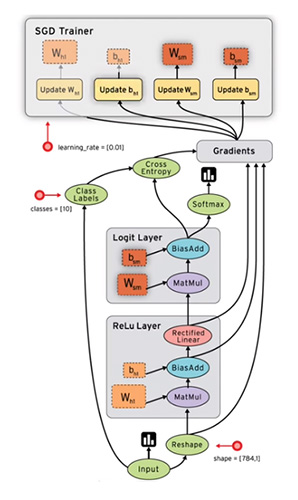
\includegraphics[width=0.5\linewidth]{img/tf-sample-graph.jpg}
	\caption{Przykładowy graf operacji}
	\label{img:tf-smpl-grf}
\end{figure}

\subsection{Konstrukcja grafu}
W pierwszym etapie tworzenia sieci neuronowej należy zdefiniować graf operacji. W~następnym kroku można wykonać
wybrane operacje, a~silnik Tensorflow sam wykona wszystkie akcje wymagane do~poprawnego obliczenia ich rezultatu.

Podczas konstrukcji grafu zamiast konkretnych danych wykorzystywane są dane symboliczne (np.~,,zmienna~x'',
,,dana~C''). Dopiero później, w~etapie wykonania operacji, za~niektóre z~owych danych podstawiane
są~odpowiednie wartości (podczas wykonywania operacji do~silnika Tensorflow podawany jest tzw.~kontekst będący
słownikiem odwzorowującym wybrane dane symboliczne na~realne wartości).

\pythonexternal{code/graph_creation.py}

\subsection{Wykonanie operacji}
Dwoma naistotniejszymi operacjami wykonywanymi podczas konstrukcji sieci neuronowej będą:
\begin{itemize}
    \item operacja uczenia,
    \item operacja klasyfikacji.
\end{itemize}

Mając już skonstruowany graf operacji, można wykonać dowolną operację zdefiniowaną w~grafie (np.~operację klasyfikacji).

\pythonexternal{code/op_execution.py}
